\scanpage{6}
% source lines 1-2
Soit $K$ un corps de nombres fini sur $\mathbb Q$.

Pour toute place $\mathfrak p$ de $K$ (finie ou infinie), on considère
\[
\left\{\begin{aligned}
&K_{\mathfrak p}\ \text{corps local de }\mathfrak p\quad(\approx\mathbb R\text{ ou }\mathbb C\text{ si }\mathfrak p\text{ est infini})\\
&U_{\mathfrak p}\ \text{ens des éléments de }{\unsure{U|K}}_{\mathfrak p}\text{ tels que }|a|_{\mathfrak p}=1\quad(\text{unités de }\mathfrak p)\ (\pm1\text{ ou }\mathbb T\text{ à l'infini})\\
&W_{\mathfrak p}=K_{\mathfrak p}^*/U_{\mathfrak p}\quad\text{groupe des valeurs}\quad(\mathbb Z:\text{\unsure{distance} finie},\mathbb R^{*+}\text{ à l'infini})
\end{aligned}\right.
\]
\margin{\figure{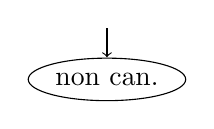
\begin{tikzpicture}\draw[->] (0,.65)--(0,.28);\draw (0,0) ellipse (1cm and .27cm);\node at (0,0) {\unsure{non can.}};\end{tikzpicture}}}

% source lines 6-8
$\bigl(\ \unsure{J|\mathscr{J}}(K)\subset\prod K_{\mathfrak p}^*$, défini comme l'image inverse de $\coprod W_{\mathfrak p}$ par $\prod K_{\mathfrak p}\longrightarrow\prod W_{\mathfrak p}$. Topologie
\inserted{(idèles)}

$\bigl(\ {\unsure{D|\mathscr{D}}}_{\mathrm{abs}}(K)=\underset{\mathfrak p}{\coprod^{\deleted{\unsure{\prod}}}}W_{\mathfrak p}$

$\bigl(\ V(K)$ (idèles unités) $=\prod U_{\mathfrak p}$, donc on a une suite exacte
\[
0\longrightarrow V(K)\longrightarrow J(K)\longrightarrow D_{\mathrm{abs}}(K)\longrightarrow0.
\]

% source lines 9-12
\deleted{\unsure{P(K)=}}\inserted{($K^*$ idèles principaux, \uline{discret} \uline{dans} $J(K)$)}

$\bigl(\ C(K)=J(K)/\deleted{\unsure{P}}K^*$ (compte tenu de l'application diagonale $K^*\longrightarrow J(K)$)
\[
0\longrightarrow K^*\longrightarrow J(K)\longrightarrow C(K)\longrightarrow0
\]

% source lines 13-15
$\bigl(\ \unsure{\mu|U}(K)=$ racines de l'unité de $K=$ torsion de
\diagram{\begin{tikzcd}[ampersand replacement=\&]K^*\unsure{\infty|\deleted{=}}\arrow[d]\\\text{\unsure{th. particulier}}\end{tikzcd}}
\margin{$P\cap V=$ unités absolues de $K$}


$\bigl(\ {\unsure{\mathscr{P}|\mathfrak{P}|\mathcal{P}}}_{\mathrm{abs}}(K)=D_{\mathrm{abs}}(K)/\operatorname{Im}K^*$ d'où

\deleted{$\unsure{E(K)}=$}
\[
0\longrightarrow\mu(K)\longrightarrow K^*\longrightarrow D_{\mathrm{abs}}(K)\longrightarrow\mathscr{P}_{\mathrm{abs}}(K)\longrightarrow0
\]

% source lines 16-18
$\bigl(\ J(K)\longrightarrow\mathbb R^{*+}$ l'hom norme déduit de $D_{\mathrm{abs}}(K)\longrightarrow\mathbb R^{*+}$,

$\bigl(\ J_0(K)$ et $D_{\mathrm{abs},0}(K)$ les idèles et diviseurs abs. de norme $1$.

On a $K^*\unsure{\in|\subset}J_0(K)$ d'où
\[
\left\{\begin{aligned}
&\mathscr{P}_{\mathrm{abs}}(K)\longrightarrow\mathbb R^{*+}\quad\text{et }\mathscr{P}_{\mathrm{abs},0}(K)\\
&C(K)\longrightarrow\mathbb R^{*+}\quad\text{et }C_0(K)
\end{aligned}\right.
\]

% source: large lower diagram
\diagram{\begin{tikzcd}[ampersand replacement=\&,column sep=small,row sep=large]
\&\&V(K)\arrow[dr,"\text{diviseurs abs. principaux}" description]\arrow[drr,"D_{\mathrm{abs},0}(K)",bend left=8]\arrow[drrr,"D_{\mathrm{abs}}(K)",bend left=13]\&\&\&\\
0\arrow[r]\&\mu(K)\arrow[ur]\arrow[dr]\&\&K^*V(K)\arrow[r,"\deleted{\unsure{\text{classes absolues}}}","\mathscr{P}_{\mathrm{abs},0}(K)"']\&J_0(K)\arrow[r,"\mathbb R^{*+}"']\&J(K)\\
\&\&K^*\arrow[ur,"\unsure{\text{ramification}}" description]\arrow[urr,"C_0(K)"',bend right=8]\arrow[urrr,"C(K)"',bend right=20]\&\&\&
\end{tikzcd}}

% source lines 19-22
\uline{Th. de Dirichlet} $C_0(K)$ est compact

La démonstration se fait par Minkowski.

Comme $K^*V(K)/K^*$ est comp., le th. \unsure{équivaut} au fait que le groupe $D_{\mathrm{abs},0}(K)/\operatorname{Im}K^*$ des classes
% archive sheet number: 5
